\documentclass{resume} % Use the custom resume.cls style

\usepackage[left=0.75in,top=0.6in,right=0.75in,bottom=0.6in]{geometry} % Document margins
\usepackage{fontawesome}
\usepackage{hyperref}
\hypersetup{
    colorlinks=true,
    linkcolor=blue,
    filecolor=magenta,      
    urlcolor=cyan,
}
\usepackage{graphicx}
% Skill bars filled proportionally
\usepackage{xcolor}
\usepackage{fancyhdr}
\usepackage{array,longtable,picture}
\definecolor{noskillgray}{gray}{0.85}
\definecolor{skilledblue}{rgb}{0.05,0.05,0.65}

\makeatletter
\newdimen\skillb@level
\newdimen\skillb@length
\newdimen\skillb@height
\skillb@length=120pt%
\skillb@height=10pt%
\newcommand*{\skillbar}[1]{%
	\skillb@level=\dimexpr#1\skillb@length/100\relax%
	{\color{skilledblue}\rule{\skillb@level}{\skillb@height}}%
	{\color{noskillgray}%
		\rule{\dimexpr\skillb@length-\skillb@level\relax}{\skillb@height}}%
}
\newcommand*{\skill}[2]{%
	\par\noindent%
	{\hskip 1ex\small #1}\\%
	\skillbar{#2}%
}
\makeatother

% -----------------------------------------------------------------------------
% \noindent % 4cm is the picture's width, -6cm by trial and error

% \begin{picture}(0,0)
% \put(\dimexpr\textwidth-4cm,-6cm){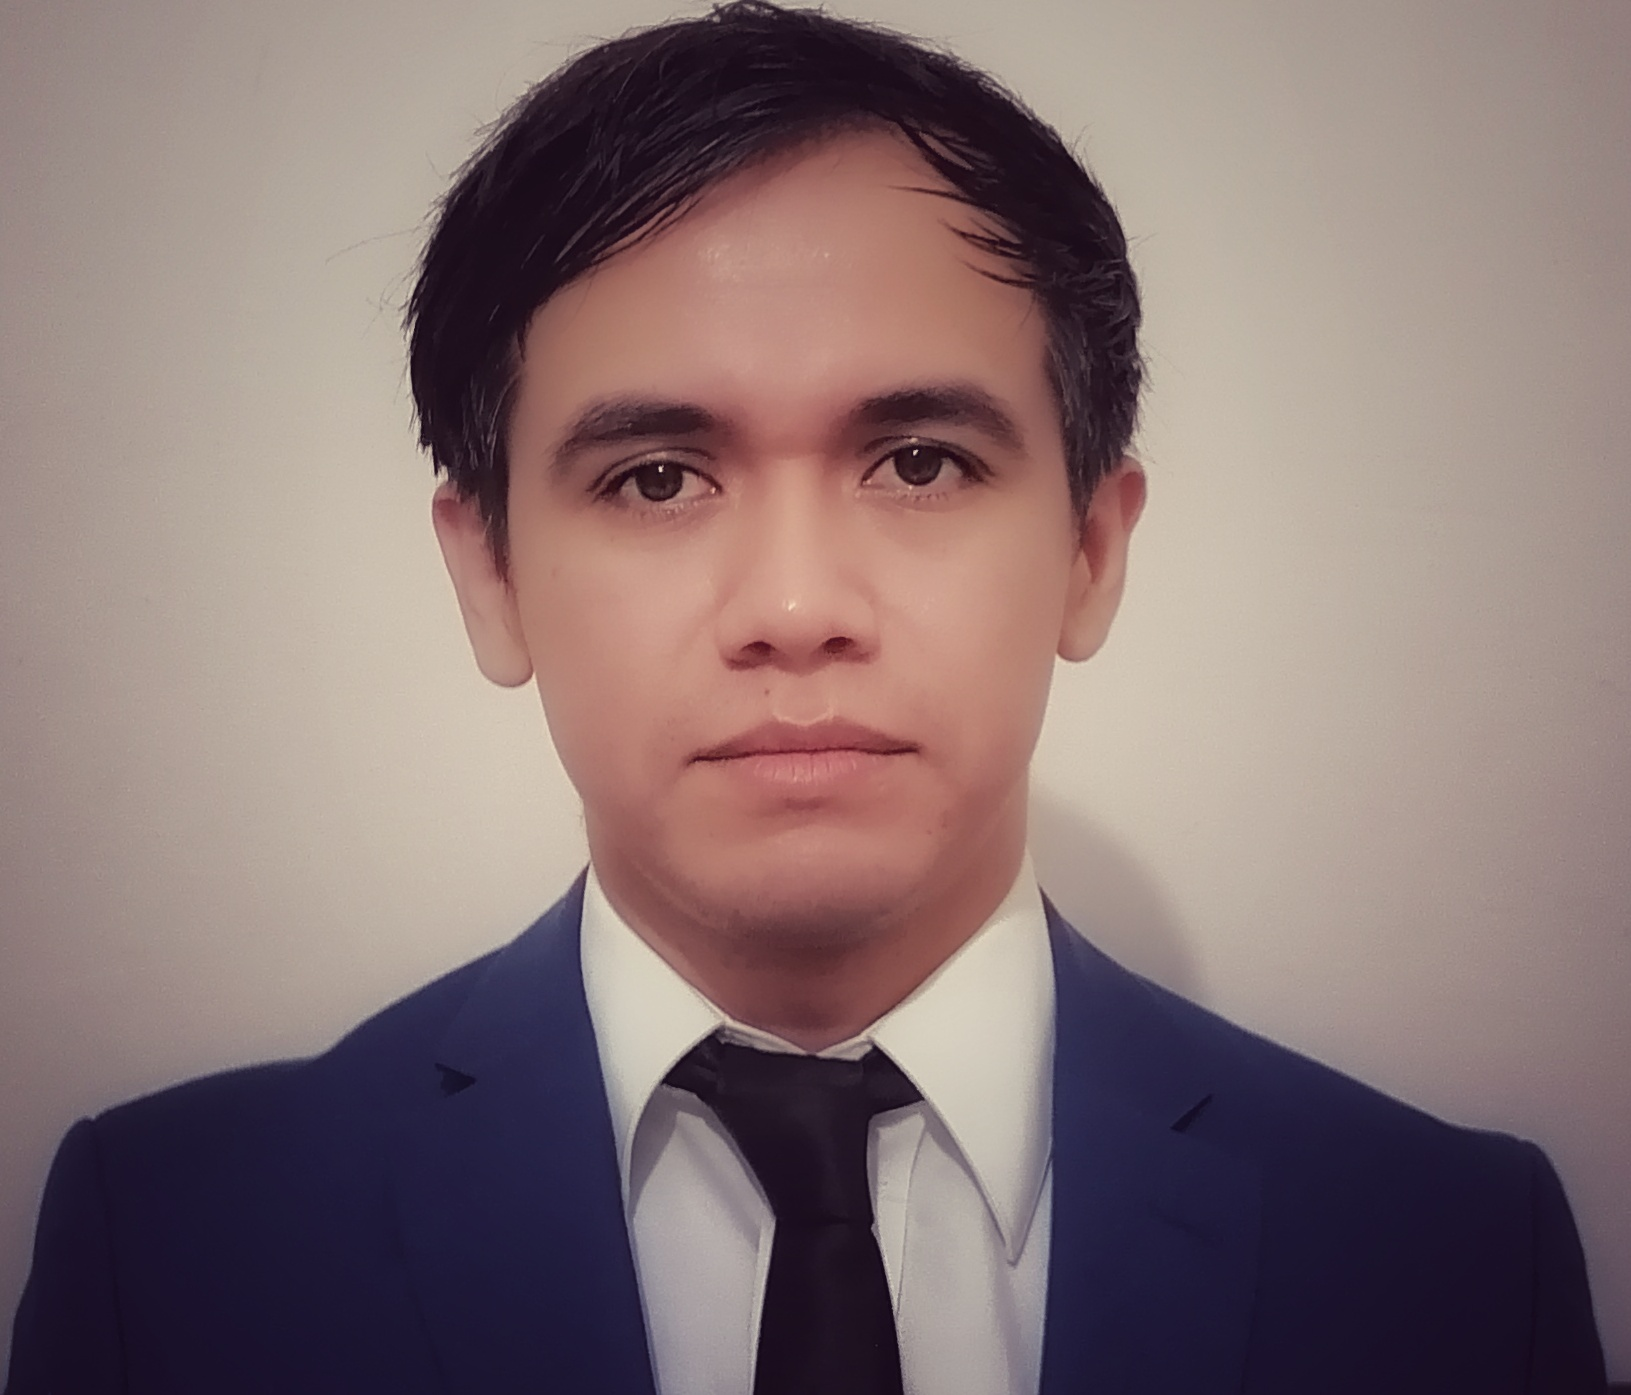
\includegraphics[width=4cm]{pic_CV.jpeg}}
% \end{picture}

\name{Emmanuel Alcalá} % Your name

%\address{123 Broadway \\ City, State 12345} % Your address
%\address{123 Pleasant Lane \\ City, State 12345} % Your secondary addess (optional)
%\address{WebPage: \url{https://jealcalat.github.io/} \tiny{\faExternalLink}} % Your phone number and email
%\address{\faMobile \hspace{1ex} {\sf 33 14 99 93 16}}

% \address{e-mail:}
\address{ \faEnvelope \hspace*{0.2em}%
                 \texttt{jealcalat@gmail.com} \\
                 \texttt{jaime.alcala@iteso.mx}}
                 
\address{\faGithub \hspace{1ex} \url{https://github.com/jealcalat}}

\address{Web (spanish): \faGlobe \hspace{1ex} \url{https://jealcalat.github.io/}}

\begin{document}
% \thispagestyle{fancy}

% \makecvheader

\begin{picture}(0,0)
    \put(0,-9){\fbox{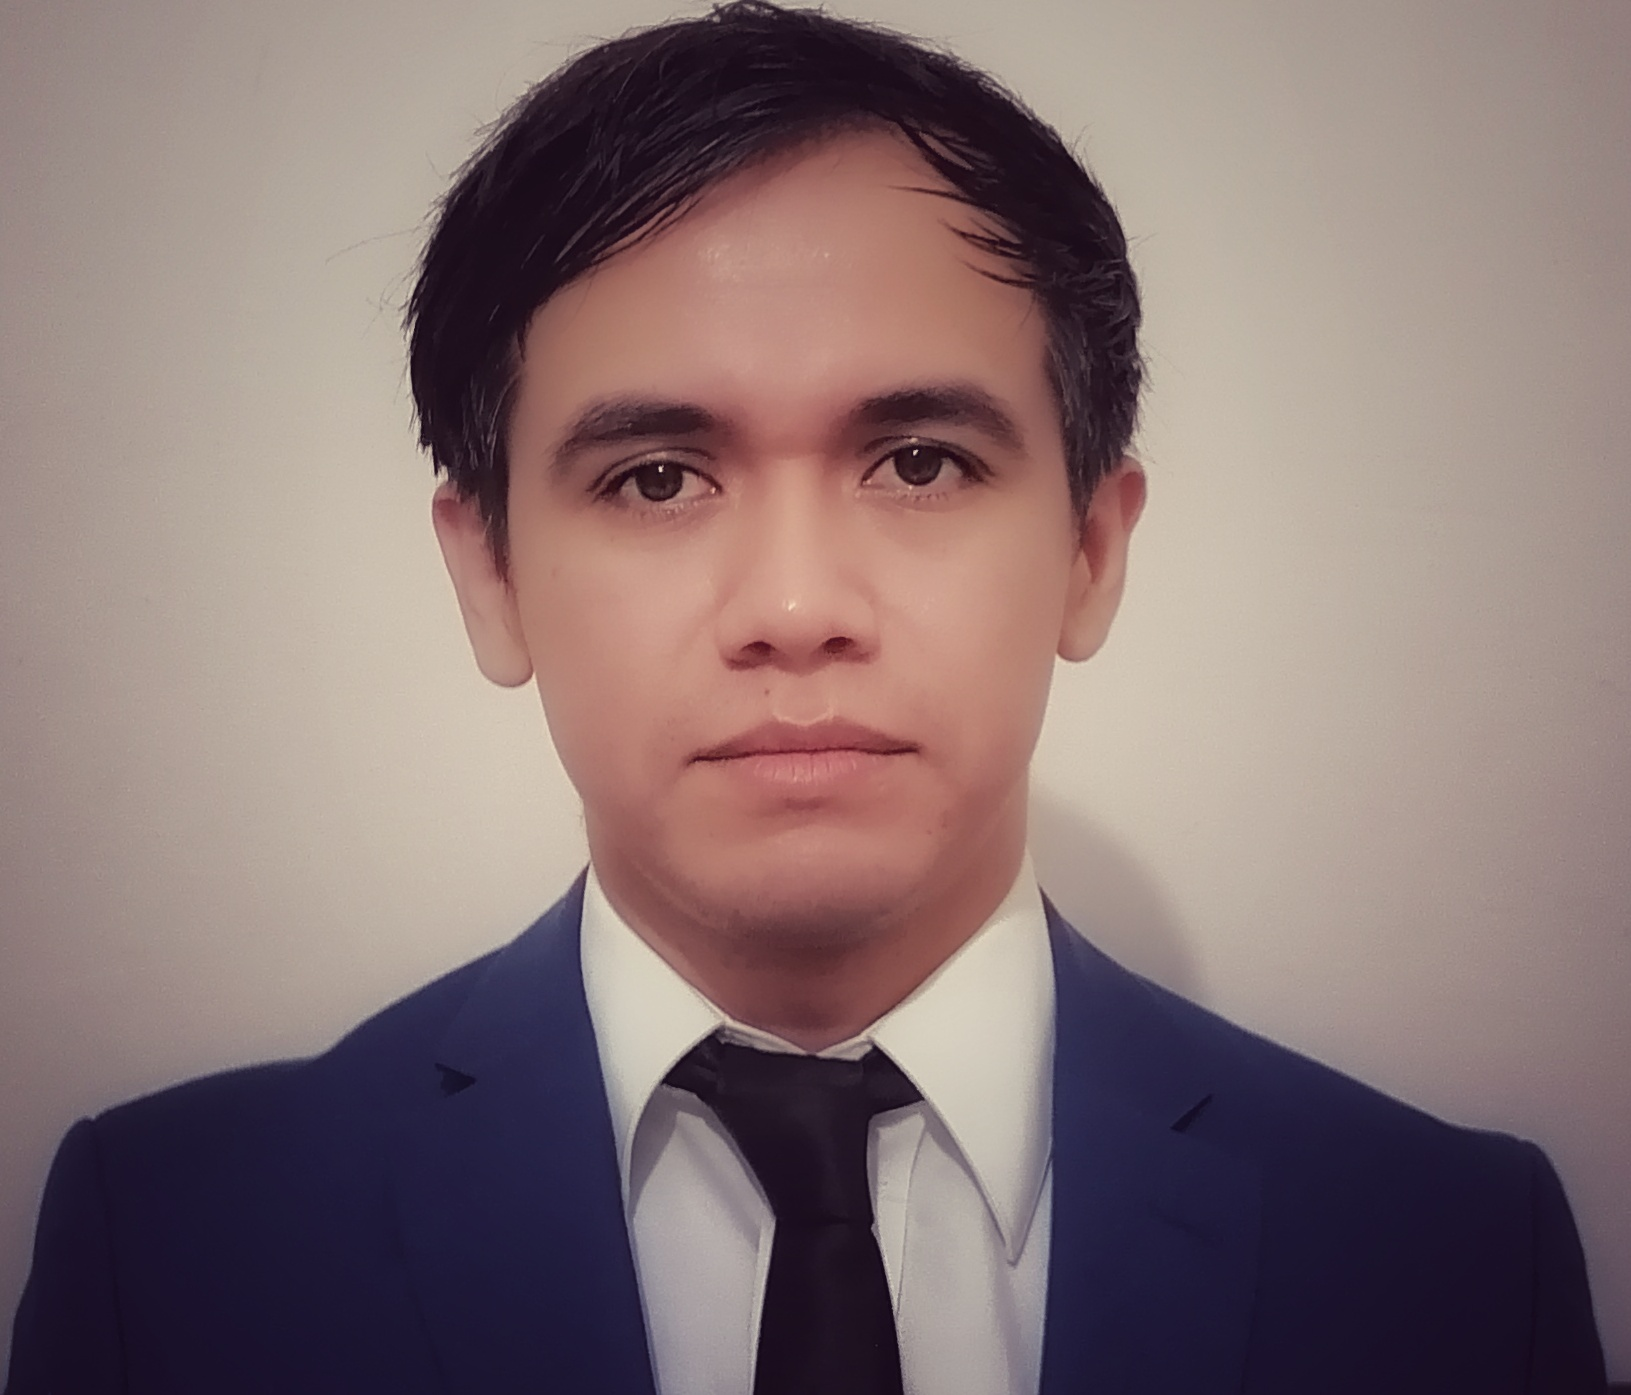
\includegraphics[width=10em]{pic_CV.jpeg}}}
\end{picture}

% \begin{flushright}
% 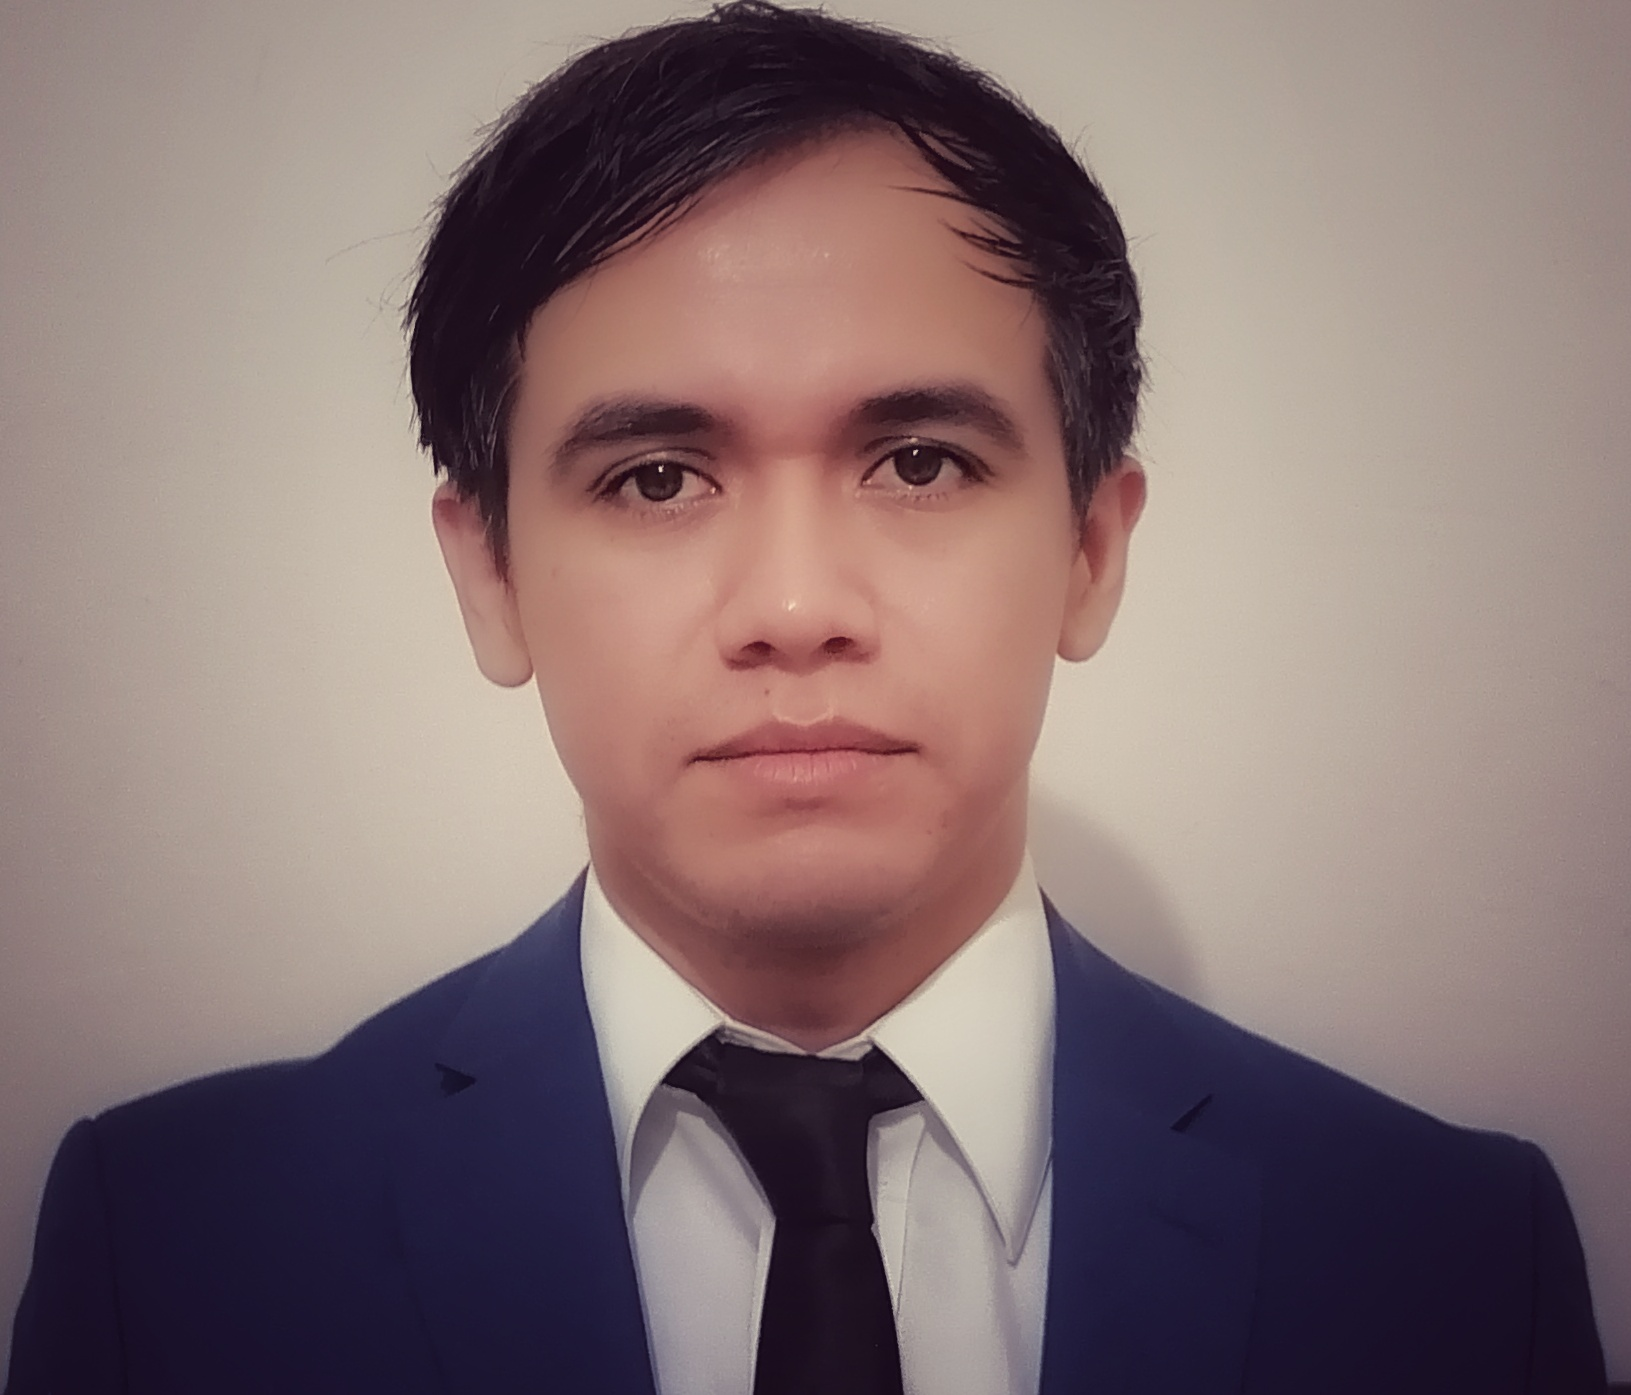
\includegraphics[scale=0.05]{pic_CV.jpeg}
% \end{flushright}

\begin{rSection}{About me}

5+ years of experience modeling real-world phenomena to answer research questions and optimize processes. During my PhD and MSc, I built expertise in computationally modeling economic behavior using neural networks and probabilistic models. I thrive in diverse settings, employing both hypothesis-driven and data-driven approaches to unravel complex questions. My passion lies in applying AI to quantitatively study and model phenomena across scientific and applied domains.

Leveraging my expertise in design of experiments and response surface methodology, I optimized nanosensor fabrication as posdoctoral researcher at ITESO (a private higher education institute in Mexico), reducing cost fabrication with faster turnaround for industrial applications. Teaching responsibilities included courses on Decision Making, Game Theory, and Econometrics for Financial Engineering, and currently Advanced Statistical Analysis for the Master of Data Science. 

Following a three-month research assistantship at Panamerican University, I transitioned to a postdoctoral research role at the University of Guadalajara in 2022, where I honed my Python and R programming skills to create \href{https://github.com/jealcalat/YEAB}{YEAB}, an open-source R package. This experience exemplifies my ability to translate complex concepts into practical applications while continuously expanding my skillset through challenging projects. Throughout my scientific career, I've authored peer-reviewed articles, effectively communicating intricate ideas to diverse audiences and engaging in collaborative, creative environments that demand assertive communication and critical thinking.

\end{rSection}

\begin{rSection}{Education}

{\bf University of Guadalajara} \hfill {\em 2008 - 2012} \\
Bachelor of Pharmaceutical Chemistry \\
% Thesis: GMOs and standardization of Western-Blot \
{\bf University of Guadalajara, CEIC-CUCBA} \hfill {\em 2015 - 2017} \\
Master of Behavioral Sciences \\
Examination Date: July 6, 2017\\
Thesis: Neural network model of impulsive choice \\
{\bf University of Guadalajara, CEIC-CUCBA} \hfill {\em 2017 - 2021} \\
Doctor of Behavioral Sciences \\
Examination Date: May 24, 2021\\
Thesis: Habit formation and resistance to change; computational models

\end{rSection}

\begin{rSection}{Experience}

\begin{rSubsection}{University of Guadalajara (UdG)}{Dec 2022-}{Posdoctoral Researcher}{}

\item Data analysis of spatial data.
\item Design of experiments.
\item Data wrangling.
\item Neural network modeling of multivariate series data with deep variational autoencoders.
\end{rSubsection}

\begin{rSubsection}{Panamerican University (UP)}{Jul 2022 - Nov 2022}{Research Assistant}{CONAHCyT - Project 320943}

\item Data wrangling.
\item Feature engineering.
\item Data analysis.
\item Writing and testing an R package (see \href{https://github.com/jealcalat/YEAB}{YEAB}).
\end{rSubsection}

\begin{rSubsection}{ITESO}{2021}{Research Assistant}{COECYTJAL - Project FODECYJAL 8248-2019}

\item Design of Experiments, Regression Analysis, DataViz, Response Surface Methodology.
\end{rSubsection}

\begin{rSubsection}{ITESO}{2021-}{Associate Professor}{}
    \item Game Theory and Decision Making in Financial Engineering
    \item Econometrics.
    \item Advanced Statistical Analysis.
\end{rSubsection}

\begin{rSubsection}{University of La Ciénega}{2019}{Lecturer}{Guadalajara, Jal}
\item BioStatistics for Nutritionists
\end{rSubsection}

\begin{rSubsection}{Consultant (Freelancer)}{2018 - }{Data Analysis and Statistical Consulting}{Guadalajara, Jal}
\item Experimental design, data analysis, and statistical inference for decision-making
\item Example project: San Javier Hospital, Fistula Day: \url{https://bit.ly/2Vz2sl7}
\end{rSubsection}

\begin{rSubsection}{UTEG}{2017}{Academic Advisor}{Guadalajara, Jal}
\item Advisor and mentor for talented students.
\end{rSubsection}

\end{rSection}

\begin{rSection}{Skills {\normalfont (0 - 100 \%)}}

\begin{tabular} { @{} >{\bf}l @{\hspace{6ex}} l }
	\skill{\sf R \& RStudio (IDE)}{70} & Language, statistical software, and various libraries \\
	\skill{\sf Python 3}{45} & Language, OpenCV, and data science libraries\\
	\skill{\LaTeXe}{65} & Preparation of scientific and technical documents \\
	\skill{Linux}{75} & OS (different distros) and basic shell scripting \\
    \skill{Windows}{70} & OS and MS Office suite \\
    \skill{macOS}{50} & OS and basic shell scripting 
\end{tabular}

\end{rSection}

\begin{rSection}{Additional Education}
	{\em 2016}  \\
	{\bf Probability Theory and Mathematical Statistics for Physicists} \hfill {\em CUCEI, UdG}
	
	{\bf Data Science Bootcamp (In-person)} \hfill {\em IBM-UdG}

	{\em 2017} \\
	{\bf Model Comparison in Quantitative Analysis of Behavior} \hfill {UAA - Randolph Grace, PhD} 
	
	{\bf Linear Algebra Course} \hfill {\em CUCEI, UdG}
	
\end{rSection}

\begin{rSection}{Distinctions}

{\bf National System of Researchers - C.} {\em 2022 - 2025}\\

\end{rSection}


\begin{rSection}{Some publications}

{\em 2019} \\
Buriticá, J.J., \& \textbf{Alcalá, E.} (2019). Increased Generalization in a Peak Procedure after Delayed Reinforcement. \textit{Behavioural Processes, 169, 103978}.

Gómez, E. G., García, V. I., Morales, C. S., López, F. A. L., \& \textbf{Alcalá, E.} (2020). \textit{Manual de Análisis de Datos de Descuento Temporal en RStudio (MADDTeR)}. Red Universitaria de Aprendizaje (RUA) de la UNAM. \url{https://www.rua.unam.mx/portal/recursos/ficha/85989}

{\em 2021} \\
López-Cárdenas, P.G, \textbf{Alcalá, E.}, Sánchez-Torres, J.D., Araujo, E. (2021). Enhancing the Sensitivity of a Class of Sensors: A Data-Based Engineering Approach. \textit{2021 IEEE 21st International Conference on Nanotechnology (NANO)}, 221-224, DOI: \url{10.1109/NANO51122.2021.9514352}. 

López-Cárdenas, P. G.,\textbf{ Alcalá, E.}, Sánchez-Torres, J. D., \& Araujo, E. (2021, November). A Resampling Approach for the Data-Based Optimization of Nanosensors. In \textit{2021 18th International Conference on Electrical Engineering, Computing Science and Automatic Control (CCE) (pp. 1-4). IEEE.}

{\em 2022}\\ 
Campos-Ordoñez, T.,\textbf{Alcalá, E.}, Ibarra-Castañeda, N., Buriticá, J., González-Pérez, 0. (2021). A repeated cyclohexane inhalation generates stereotypic circling, hyperlocomotion, persistent anxiety-like behavior, and dysregulates the c-Fos expression in striatum and nucleus accumbens. \textit{Behavioural brain research, 418, 113664}

Sosa, R., \textbf{Alcalá., E}. (2022). The Nervous System as a Solution for Implementing Closed Negative Feedback Control Loops. \textit{Journal of Experimental Analysis of Behavior}, 1-22

{\em 2023}\\
López-Cárdenas, P. G.,\textbf{ Alcalá, E.}, Sánchez-Torres, J. D., \& Araujo, E. (2023). Improving self-supported nanowire arrays using response surface methodology for the synthesis of a H$_2$O$_2$ nanostructured sensor. \textit{Materials Chemistry and Physics, 303, 127729}

\end{rSection}

\end{document}
